%%%%%%%%%%%%%%%%%%%%%%%%%%%%%%%%%%%%%%%%%%%%%%%%%%%%%%%%%%%%%%%%%%%%%
%%                                                                 %%
%% Please do not use \input{...} to include other tex files.       %%
%% Submit your LaTeX manuscript as one .tex document.              %%
%%                                                                 %%
%% All additional figures and files should be attached             %%
%% separately and not embedded in the \TeX\ document itself.       %%
%%                                                                 %%
%%%%%%%%%%%%%%%%%%%%%%%%%%%%%%%%%%%%%%%%%%%%%%%%%%%%%%%%%%%%%%%%%%%%%

\documentclass[pdflatex,sn-mathphys]{sn-jnl}% Basic Springer Nature Reference Style/Chemistry Reference Style

%%%% Standard Packages and macros (don't forget to paste the macros in
%%%% the main at the end of the writing).
\usepackage{todonotes}
\usepackage{lstvhdl}
%%%%%%%%%%%%%%%%%%%%%%%%%%%%%%%%%%%%%%
%%%%%%% Misc. macros and defs. %%%%%%%
%%%%%%%%%%%%%%%%%%%%%%%%%%%%%%%%%%%%%%

% Macro definitions.

\def\bbook{\textsf{B}-Book}
\def\bmth{\textsf{B}}
\def\cakeml{\textsf{CakeML}}
\def\cnrs{\textsf{CNRS}}
\def\coq{\textsf{Coq}}
\def\java{\textsf{Java}}
\def\hilecop{\textsf{HILECOP}}
\def\inria{\textsf{Inria}}
\def\isahol{\textsf{Isabelle/HOL}}
\def\isa{\textsf{Isabelle}}
\def\hol{\textsf{HOL}}
\def\ccert{\textsf{CompCert}}
\def\lirmm{\textsf{LIRMM}}
\def\lustre{\textsf{Lustre}}
\def\nasa{\textsf{NASA}}
\def\um{\textsf{Universit\'e de Montpellier}}
\def\neurin{\textsf{NEURINNOV}}
\def\uml{\textsf{UML}}
\def\vhdl{\textsf{VHDL}}
\def\hvhdl{$\mathcal{H}$-\textsf{VHDL}}
\def\lwidth{\dimexpr\linewidth-2\fboxsep-2\fboxrule}
\def\ocaml{\textsf{OCaml}}

%%% Local Variables:
%%% mode: latex
%%% TeX-master: "main"
%%% End:

%%%%

\jyear{2022}%

%% as per the requirement new theorem styles can be included as shown below
\theoremstyle{thmstyleone}%
\newtheorem{theorem}{Theorem}%  meant for continuous numbers
%%\newtheorem{theorem}{Theorem}[section]% meant for sectionwise numbers
%% optional argument [theorem] produces theorem numbering sequence instead of independent numbers for Proposition
\newtheorem{proposition}[theorem]{Proposition}% 
%%\newtheorem{proposition}{Proposition}% to get separate numbers for theorem and proposition etc.

\theoremstyle{thmstyletwo}%
\newtheorem{example}{Example}%
\newtheorem{remark}{Remark}%

\theoremstyle{thmstylethree}%
\newtheorem{definition}{Definition}%

\raggedbottom
%%\unnumbered% uncomment this for unnumbered level heads

\begin{document}

\title[Formal verification of the \hilecop{} methodology]{Formal verification of a methodology for the design and
  production of safety-critical digital systems}

%%=============================================================%%
%% Prefix	-> \pfx{Dr}
%% GivenName	-> \fnm{Joergen W.}
%% Particle	-> \spfx{van der} -> surname prefix
%% FamilyName	-> \sur{Ploeg}
%% Suffix	-> \sfx{IV}
%% NatureName	-> \tanm{Poet Laureate} -> Title after name
%% Degrees	-> \dgr{MSc, PhD}
%% \author*[1,2]{\pfx{Dr} \fnm{Joergen W.} \spfx{van der} \sur{Ploeg} \sfx{IV} \tanm{Poet Laureate} 
%%                 \dgr{MSc, PhD}}\email{iauthor@gmail.com}
%%=============================================================%%

\author*[1]{\fnm{Vincent} \sur{Iampietro}}
\author[1]{\fnm{David} \sur{Delahaye}}
\author[1,2]{\fnm{David} \sur{Andreu}}

\email{Firstname.Lastname@lirmm.fr}
\email{David.Andreu@neurinnov.com}

\affil*[1]{\orgname{\lirmm, \um, \cnrs},
  \city{Montpellier}, \country{France}}

\affil[2]{\orgname{\neurin}, \city{Montpellier}, \country{France}}

\abstract{}

\keywords{}

\maketitle

\listoftodos

\section{Introduction}
\label{sec:intro}

The domain of Model-Based Systems Engineering (MBSE) \cite{Long2011}
proposes a framework to help engineers to design and produce digital
systems, in a well-documented, safe and reliable way. Comparable to
what Model Driven Engineering (MDE) does in the world of software
engineering, models are first order concepts in MBSE.  As illustrated
in Figure~\ref{fig:MBSE-ps}, a MBSE process describes a way to design
a digital system starting from a high-level view of the system. This
high-level view can follow a graphical formalism such as SysML
\cite{Friedenthal2014} or Petri nets (PNs) \cite{Petri1962}, or a
textual one such as SystemC \cite{Black2009} or VHDL
\cite{Ashenden2010}. Then, the MBSE process describes many refinements
phases (the downward-going green arrows in Figure~\ref{fig:MBSE-ps})
during which the input model will be transformed; at each refinement
phase, the model goes down in abstraction towards its final
implementation as a hardware circuit. A refinement phase, which is
also a transformation phase, can be performed automatically or
manually.

\begin{figure}[H] \centering
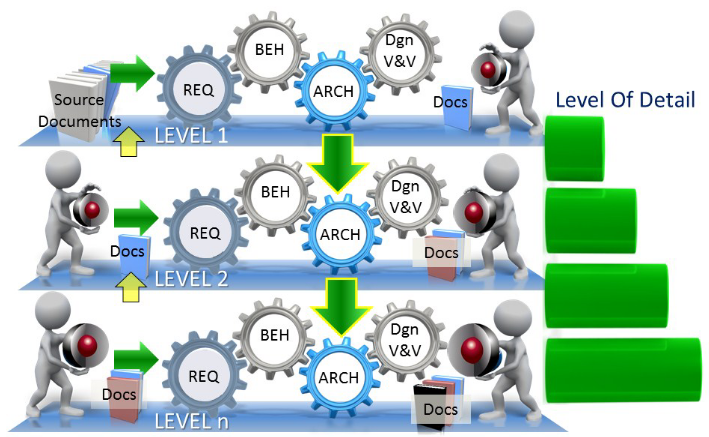
\includegraphics[keepaspectratio,width=.7\textwidth]{MBSE-ps.png}
  \caption[A Model-Based Systems Engineering process.]{A Model-Based
Systems Engineering process; REQ stands for requirements, BEH for
behavior, ARCH for architecture, Dgn V\&V for design verification and
validation. This figure is an excerpt from \cite{Long2011}.}
  \label{fig:MBSE-ps}
\end{figure}

In the case where the digital system being designed is a
safety-critical system, an MBSE process will often employ formal
models as the design formalism. Thus, these models enable a certain
extent of mathematical reasoning to prove that safety properties are
met during the design V\&V phase (cf. Figure~\ref{fig:MBSE-ps}).

To assist the engineers in the design and the implementation of
safety-critical digital systems, the CAMIN team came up with a process
called the ``\hilecop{} methodology'' \cite{Andreu2009}.  This
methodology follows the principles of a MBSE process and relies on
several transformations going from abstract models to concrete FPGA
(Field-Programmable Gate Array) or ASIC (Application-Specific
Integrated Circuit) implementations through the production of VHDL
code. Figure~\ref{fig:hilecop-wf} details the global workflow of
\hilecop{}.

\begin{figure}[H]
\centering
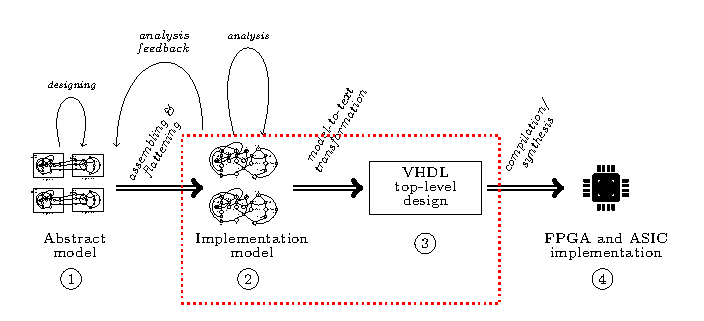
\includegraphics[keepaspectratio=true,width=\textwidth]{hilecop-wf.eps}
\caption[Workflow of the \hilecop{} methodology.]{Workflow of the
  \hilecop{} methodology; horizontal double arrows indicate the
  transformation phases, i.e. the refinement phases in MBSE terms;
  simple arrows indicate different kinds of operations performed at a
  given step.}
\label{fig:hilecop-wf}
\end{figure}

In Figure~\ref{fig:hilecop-wf}, Step~1 corresponds to the design phase
of a digital system. At this step, the user produces a model of the
required system; the leveraged model formalism is a graphical
formalism based on component diagrams and specific Petri nets (PNs).
In Figure~\ref{fig:hilecop-wf}, the transformation from Step~1 to
Step~2 flattens the model. The internal behaviors of separate
components are connected according to the interface compositions, and
embedding component structures are removed. The result of this
transformation step is a global PN that represents the internal
behavior of the digital system.  The class of PNs used in \hilecop{}
has been specifically devised for the design of safety-critical
digital systems; a first thesis has formalized the execution semantics
of these PN models \cite{Leroux2014}. % What makes them a very
% particular kind of models is their \textit{synchronous} execution
% semantics. This semantics denotes from the standard
% \textit{asynchronous} execution of PNs.
Due to its mathematical
foundations, a PN model can be analyzed, and a proof that a given
model meets some properties can be automatically produced through the
direct analysis of the structure or through the use of model-checking
techniques. This feature of PNs has been one of the reason of the
adoption of this formalism as \hilecop{}'s base formalism. A thesis
has been dedicated to the development of new methods to analyze the
\hilecop{} PN models \cite{Merzoug2018}. The analysis phase is here to
convince the engineers that they are indeed designing a safe
system. The analysis process is a round trip between Step~1 and
Step~2.  It aims at producing a model that is conflict-free (see
Section~\ref{sec:hilecop-models} for more details about the definition
of a conflict), bounded, and deadlock-free, using model-checking
techniques.  After several iterations, the model should reach
soundness and is then said to be \emph{implementation-ready}.

In Figure~\ref{fig:hilecop-wf}, from Step~2 to Step~3, \vhdl{} source
code is then generated by means of an automatic model-to-text
transformation. The generated code describes a \vhdl{} design, i.e. a
textual description of a hardware system, which has an interface
defining input and output ports and an internal behavior called an
architecture.

From Step~3 to Step~4, the \vhdl{} compilation/synthesis and the FPGA
programming, or ASIC realization, are finally performed using
industrial tools. At the end of Step~4, the designed circuit is
physically built on an FPGA device or an ASIC.  What happens between
Step~3 and Step~4 appears as a black box in the whole \hilecop{}
methodology. Therefore, we will not consider this transformation
phase, which will not be verified.

\subsection{Verifying the \hilecop{} methodology}
\label{sec:verif-hilecop}

The use of Petri nets as a base model is one of the major advantage of
the \hilecop{} methodology. All the analysis tools that accompany the
Petri net formalism, and allow us to prove that the models meet some
required properties, qualify the \hilecop{} methodology as a formal
method for the design and implementation of safety-critical digital
systems. However, the advantages provided by the use Petri nets would
be lost if one of the transformations performed during the process
changes the input model in a way that would alter its behavior. Thus,
the engineers would have specified a perfectly correct digital system
but would never obtain the expected circuit on a physical device. In
order to reinforce the confidence in the \hilecop{} methodology, the
goal of our work is to verify, by establishing a formal proof, that
the model-to-text transformation from Step~2 to Step~3 (i.e. the
framed part with red dotted lines in Figure~\ref{fig:hilecop-wf})
preserves the behavior of the input models into the generated \vhdl{}
designs. We choose to carry out this task as a deductive verification
task.  We aim at proving a theorem stating that the \hilecop{}
model-to-text transformation is \textit{semantic-preserving}. This
theorem will be of the following form: for all PN model, input to the
\hilecop{} transformation, the generated output \vhdl{} design behaves
similarly at execution time. Section~\ref{sec:proof} formally presents
our behavior preservation theorem, and thus, what we mean about the
similarity of execution between a PN model and a \vhdl{} design.

One could argue that to qualify the entire \hilecop{} methodology, one
has to verify all the transformations used in the methodology,
i.e. consider also the transformation from Step~1 to Step~2, and the
transformation from Step~3 to Step~4. However, we shall say that:

\begin{itemize}
\item The transformation from Step~1 to Step~2 changes the structure
  of the component-based input model. Even if the removal of the
  component structures induces some structural rearrangements, the
  behavior of the flattened model is almost similar to the one of the
  component-based model. Therefore, we argue that verifying that this
  transformation is semantic-preser\-ving is an easy enough task.

\item The transformation from Step~3 to Step~4 is performed by
  industrial tools. We rely on these tools because they are widely
  used in the industry for the development of safety-critical systems
  (e.g. cadence tools in aerospace and defense domains). Moreover, the
  compiler/synthesizer used at this stage of the methodology is a
  proprietary product. Thus, we don't have any access to the code of
  this program. % Moreover, the compiler/synthesizer performs a lot of
  % optimizations over the input \vhdl{} code. Even with a provided
  % access to the code, verifying such an optimizing compiler would not
  % possible within the time-span of this thesis.
\end{itemize}

% Now that we have clarified the nature of the verification task we want
% to achieve, we can state our research question as follows:

% \begin{center}
%   \textsc{Can we prove that the model-to-text transformation described
%     in the \hilecop{} methodology is semantic preserving?}
% \end{center}

\subsection{Related work}
\label{sec:related-work}

The verification task we want to achieve is really close to the formal
verification of compilers for programming languages. Compiler
verification has been widely explored, and many works are accessible
in the literature \cite{Dave2003}. The major source of inspiration of
this work has been the work done on the \ccert{} certified C compiler
\cite{Leroy2009}. Thus, we argue here that the scientific interest of
our research comes from the comparison between the methods used to
perform our verification task and the methods used to perform similar
verification task in other domains such as compiler verification. The
following research questions arises:

\begin{itemize}
\item What are the similarities and the differences between the
  \hilecop{} transformation and other transformation situations
  (compilers, model transformations\dots)?
\item Is there a strategy to perform the verification of the
  \hilecop{} transformation?
\item How far the correspondence holds between this strategy and the
  strategy used in other transformation situations such as compiler
  verification?
\end{itemize}

To achieve the formal verification of \hilecop{}, our approach is
similar to what has been done for the \ccert{} compiler. The idea is
to formalize the semantics of the source and target languages, and
verify that the transformation preserves the semantics of any input
model. In the thesis, we propose both to perform the formalization
work on ``paper'' and mechanize it within the \coq{} proof assistant
\cite{Bertot2004}.

In the case of \hilecop{}, some specificities of the source and target
languages introduce additional technical difficulties in the process
of formal verification. A first difference pertains to \hilecop{}'s
high-level formalism (the input language), which is quite
abstract. This formalism depends on PNs, and thus is not a common
programming language.

A second difference is about the \vhdl{} language (the output
language).  Similarly to the PN models used in \hilecop{}, the \vhdl{}
language is not a common programming language as its purpose is both
the structural and behavioral description of hardware
circuits. % Although previous work has been conducted toward the
% formalization of the \vhdl{} semantics \cite{Kloos2012}, a semantics
% that is able to both handle all the constructs in the generated
% programs, and facilitate the proof of behavior preservation, still
% needs to be designed.

\todo[inline]{ Here put the literature review.}

To further motivate the necessity of the verification task, the
development of neuroprostheses by the INRIA CAMIN team is at the base
of the creation of the Neurrinov
company\footnote{\url{http://neurinnov.com/}}. The Neurrinov company
is now looking towards the industrial development of such
neuroprostheses. We hope that once the verification performed on the
\hilecop{} methodology, it will help to obtain the CE certification,
related to the EU 2017/745 regulation text, necessary to qualify the
neuroprostheses as eligible for the medical market.

Moreover, the \hilecop{} methodology comes with a working
implementation based on the Eclipse framework . This software is
currently used by the engineers of the Neurinnov company to design the
digital systems having a part in safety-critical implantable medical
devices.

To the purpose of formal verification, we will implement the
\hilecop{} model-to-text transformation leveraging the functional
language of the \coq{} proof assistant. However, after the
mechanization of the proof of semantic preservation, we could use the
extraction feature of the \coq{} proof assistant to produce the
implemented transformation as an \ocaml{} program. Then, we will be
able to connect this program to the existing \hilecop{} software in
order
to use the verified version of the transformation.\\

This article is structured as
follows. Section~\ref{sec:hilecop-models} presents the specific kind
of Petri net models which are the input models of \hilecop{}'s
model-to-text transformation.  Section~\ref{sec:hvhdl} gives a formal
definition of the syntax and semantics of a subset of the \vhdl{}
language that we call \hvhdl{}. \hvhdl{} is the target language of the
programs generated by \hilecop{}'s model-to-text transformation.
Section~\ref{sec:m2t} presents the algorithm of the transformation and
its implementation with the \coq{} proof assistant.
Section~\ref{sec:proof} details the semantic preservation theorem
expressing that the \hilecop{} transformation is semantic-preserving.
It also gives the high-level theorems and lemmas involved in the proof
of the semantic preservation theorem.  Finally,
Section~\ref{sec:concl} ends the article, and outlines the
perspectives regarding the full completion of the task of proving that
the \hilecop{} transformation is semantic-preserving.

\section{Models of digital systems in \hilecop{}}
\label{sec:hilecop-models}

Let us introduce the input formalism of \hilecop{}'s model-to-text
transformation: Synchronously executed, extended, generalized,
Interpreted Time Petri Nets with priorities (SITPNs). The
formalization of the SITPN structure and semantics is mainly the
result of two Ph.D. theses \cite{Leroux2014,Merzoug2018}. We made a
preciser definition of both the SITPN structure and its semantics,
where precision is needed for the purpose of the proof, and
implemented them in \coq{}. Moreover, we added complementary
definitions, concerning the well-definition of an SITPN input model,
that are required to express our semantic preservation theorem. In
this section, we assume that the reader has some knowledge of the
Petri net formalism and its semantics, so that words like firing, or
marking, need no explanation. For more information on the topic of
Petri nets, the reader can refer to \cite{David1994},
\cite{Murata1989}, or \cite{Diaz2001}.

\begin{figure}[H]
\centering
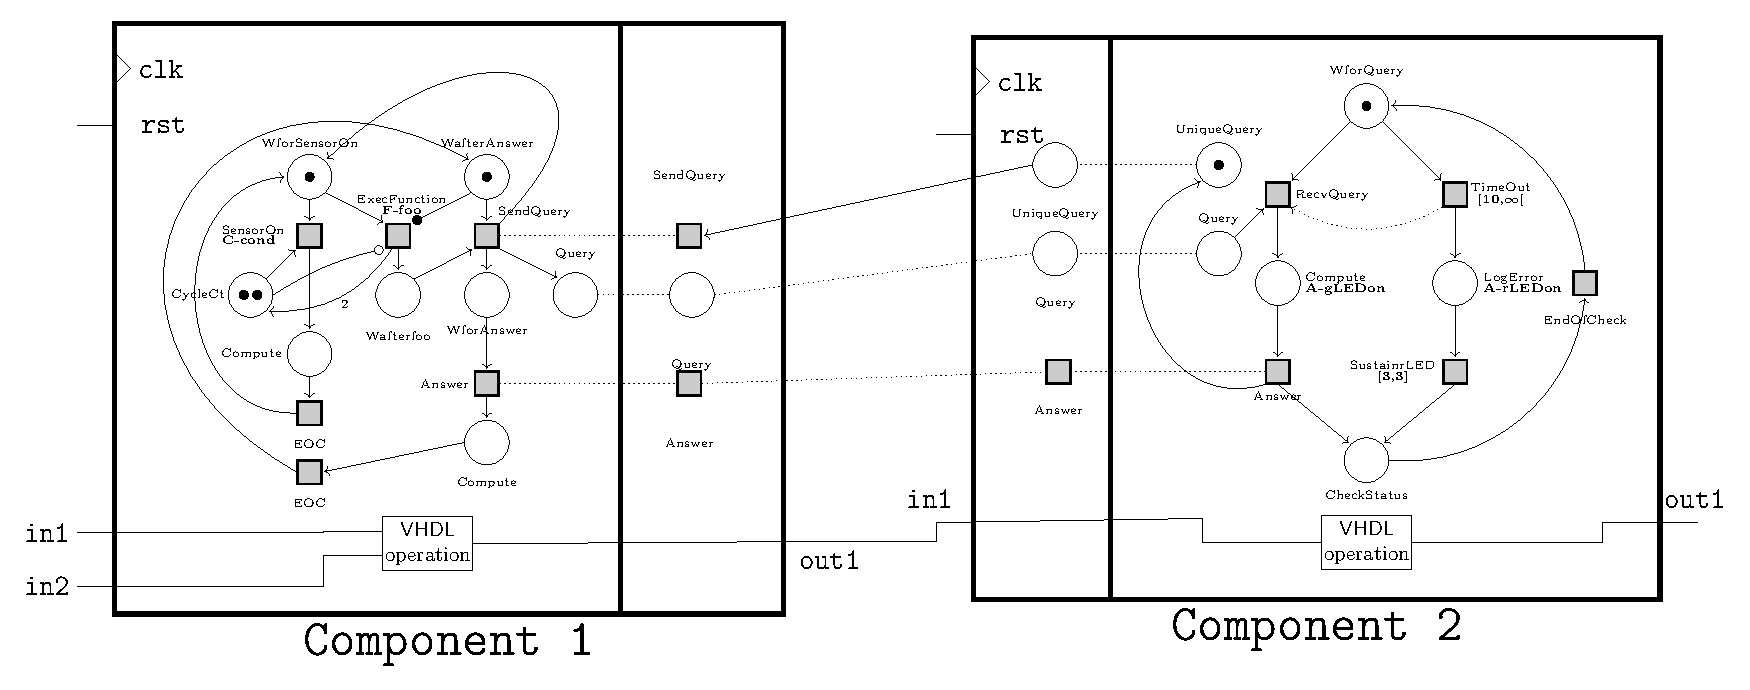
\includegraphics[keepaspectratio=true,width=\textwidth]{abs-model.eps}
\caption[An example of model of digital system in \hilecop{}.]{A
  component-based model of digital system in \hilecop{}.}
\label{fig:abs-model}
\end{figure}

In \hilecop{}'s high-level formalism, a model of digital system is
composed of boxes that represent the different components of the
system. Figure~\ref{fig:abs-model} gives an example of such a model.
The internal behavior of each component is defined by an SITPN model.
The elements of a component's internal behavior can be connected to
the elements of another component's behavior through an interface. Two
elements are either connected through a place-transition (or
transition-place) arc, or through a fusion arc (dotted line in
Figure~\ref{fig:abs-model}). While designing a component, an engineer
can also define input and output ports in the component interface,
declare internal signals, and perform operations over the ports and
internal signals by writing \vhdl{} code. All the \vhdl{} code defined
in this way will be copied as is in the output \vhdl{} design during
the model-to-text transformation. Note that all components declare a
clock and a reset signal (cf. \texttt{clk} and \texttt{rst} in
Figure~\ref{fig:abs-model}). These signals are related to the
synchronous execution of the system in the final physical device.

Before being transformed into \vhdl{} code, the model is flattened
down. All component structures are removed, and the result is one
global SITPN model. During this flattening step, all elements that
were connected through fusion arcs are merged
together. Figure~\ref{fig:impl-model} presents the global SITPN model
resulting from the flattening of the component-based model of
Figure~\ref{fig:abs-model}.

\begin{figure}[H]
\centering
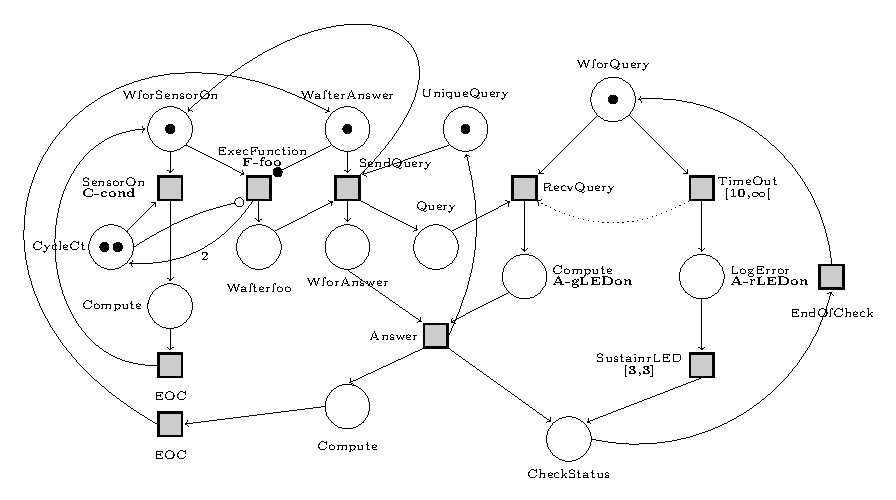
\includegraphics[keepaspectratio=true,width=\textwidth] {impl-model.eps}
\caption[Global Petri net model.]{A global Petri net model obtained
  after the flattening of a \hilecop{} high-level model.}
\label{fig:impl-model}
\end{figure}

SITPNs are a combination of multiple classes of PNs, namely: extended
PNs, generalized PNs, interpreted PNs, time PNs and PNs with
priorities. An generalized Petri net admits the weight of its arcs to
be a natural number instead of the default value of one (i.e. when no
number is written above the arc). An extended Petri net introduces two
kind of place-transition arcs, the \textit{inhibitor} arc,
characterized by a white circle head, and the \textit{test} arc, which
has a black circle head. These arcs condition the firing of a
connected transition, however, they do not cause tokens to be removed
from input places at firing time. In Figure~\ref{fig:impl-model}, the
arc from place CycleCt to transition ExecFunction is an inhibitor arc,
and the arc from place WafterAnswer to ExecFunction is a test arc.
Now, let us introduce more specifically the class of interpreted PNs,
time PNs and PNs with priorities.

\paragraph{Interpreted Petri nets}
% As stated in \cite{David1994}, Interpreted Petri Nets (IPN) ``can be
% applied to various interpretations according to the use wished to be
% made of it''.
In its general definition \cite{David1994}, an IPN is associated with
a finite set of variables $V$, a finite set of operations $O$, and a
finite set of conditions $C$. Operations of the $O$ set are associated
with places and triggered when the places become marked. The execution
of operations affects the value of the variables, and the value of
conditions depends on Boolean expressions computed upon the variables.
Conditions are associated with transitions and become involved in the
firing process.  In the \hilecop{} version of
IPNs, % refines the concepts of the general
% definition. In this version, 
the set of variables corresponds to the set of \vhdl{} signals that
are handled by the model; a signal can be an input port, an output
port or an internal signal of the modeled hardware circuit. The
operations, implemented by \vhdl{} procedures, are separated in two
kinds, namely: actions and functions. Actions (or continuous
operations) are associated to the places; all the actions associated
to a place $p$ are activated as long as $p$ is marked (i.e. as long as
$p$ holds a token). Functions (or discrete operations) are associated
to the transitions; when a transition $t$ is fired, all functions
associated to $t$ are executed once. In Figure \ref{fig:impl-model},
\textbf{C-cond} is a condition associated to the transition SensorOn;
\textbf{F-foo} is a function associated to the transition
ExecFunction; \textbf{A-gLEDon} and \textbf{A-rLEDon} are two actions
associated to the Compute and LogError places.
% Figure~\ref{fig:ipn} illustrates the use of actions, functions and
% conditions in an interpreted Petri net as applied in the \hilecop{}
% high-level models.

% \begin{figure}[H]
%   \centering
%   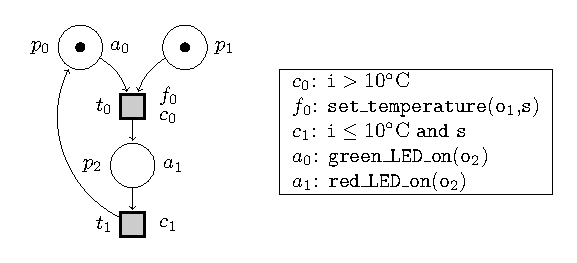
\includegraphics[keepaspectratio=true, width=.7\textwidth]{interpreted-pn.eps}
%   \caption[An example of Interpreted Petri net.]{An example of
%     interpreted Petri net; on the left side, the interpreted Petri
%     net; on the right side, examples of tests associated to conditions
%     and operations associated to actions and functions.}
%   \label{fig:ipn}
% \end{figure}%
% %
% In Figure~\ref{fig:ipn}, the set of \vhdl{} signals, on which the
% interpretation elements act upon, is
% $\{\mathit{i}, \mathtt{s}, \mathtt{o}_1, \mathtt{o}_2\}$. Here, signal
% \texttt{i} is an input port of the hardware, \texttt{s} is an internal
% signal, and \texttt{o}$_1$ and \texttt{o}$_2$ are two output
% ports. The action $a_0$ is activated as place $p_0$ is marked; thus,
% the operation \texttt{green\_LED\_on}(\texttt{o}$_2$) is currently
% executed. Also, function $f_0$ will be executed (i.e. operation
% \texttt{set\_temperature}(\texttt{o}$_1$, \texttt{s})) at the firing
% of $t_0$% , that is if condition $c_0$ is \texttt{true} and $t_0$ is
% % sensitized
% . On the right side of Figure~\ref{fig:ipn}, we associate Boolean
% expressions with conditions; these expressions depend on the value of
% the signals declared by the model. Also, we associate actions and
% functions with operations that handle the signals of the model which
% are passed as inputs. Concretely, in the \hilecop{} high-level models,
% functions and actions are declared as \vhdl{}
% procedures. Listing~\ref{lst:vhdl-fun} gives one possible
% implementation of the \texttt{set\_temperature} operation as a \vhdl{}
% procedure; the \texttt{set\_temperature} operation is associated with
% function $f_0$ in Figure~\ref{fig:ipn}.

% \begin{lstlisting}[language=vhdl,
% caption={[An example of \vhdl{} procedure implementing a function.]An example of \vhdl{} procedure implementing the operation \texttt{set\_temperature} associated with the function $f_0$.},label={lst:vhdl-fun},framexleftmargin=1.5em,xleftmargin=2em,numbers=left,numberstyle=\tiny\ttfamily]
% procedure set_temperature(signal tmp : out integer; signal flag : inout std_logic) is
% begin
%   if flag = '1' then
%     tmp <= 30;
%     flag <= '0';
%   else 
%     tmp <= 10;
%     flag <= '1';
%   endif;
% end set_temperature;
% \end{lstlisting}

% In Listing~\ref{lst:vhdl-fun}, the \texttt{set\_temperature} procedure
% declares two parameters: the \texttt{tmp} signal which is a write-only
% signal of type \texttt{integer}, and the \texttt{flag} signal which is
% a both readable and writable signal of the Boolean type
% (\texttt{std\_logic} in \vhdl{}). The \texttt{set\_temperature}
% procedure checks the value of the \texttt{flag} signal and assigns a
% new value to the \texttt{tmp} and \texttt{flag} signals
% accordingly.
% The $\Leftarrow$ operator is the assignment operator for
% signals in the \vhdl{} syntax (more on that in
% Section~\ref{sec:hvhdl}).

\paragraph{Time Petri nets}

In a time Petri net (TPN), time intervals can be associated to
transitions, along with a dynamic time counter value. Thus, the firing
of a transition must happen in a certain time window. In the
\hilecop{} version of TPNs, time intervals are of the form $[a, b]$,
where $a\in\mathbb{N}^{*}$ and
$b\in\mathbb{N}^{*}\sqcup\{\infty\}$. Other definitions of time
intervals exist for TPNs (e.g. with real numbers), but here we will
only consider the latter definition. In Figure~\ref{fig:impl-model},
transitions SustainrLED and TimeOut are both associated with time
intervals.

\paragraph{Petri nets with priorities}

Two transitions are in structural conflict if they have a common input
place connected through a \textit{basic} arc (i.e. neither inhibitor
nor test arc). When two transitions in structural conflict are firable
at the same time and if the firing of one of the transitions disables
the other, then, the conflict becomes \textit{effective}. In a Petri
net with priorities, it is possible to specify a firing priority in
the case where the conflict between two transitions becomes
effective. In that case, the transition with the highest firing
priority will always be fired first. In Figure \ref{fig:impl-model},
the fact that transition TimeOut has a higher firing priority than
transition RecvQuery is graphically represented by a dotted arrow. \\

\noindent{}Now let us formally introduce the structure of SITPNs:

\begin{definition}[SITPN]
  \label{def:sitpn}
  A synchronously executed, extended, generalized, interpreted, and
  time Petri net with priorities is a tuple
  ${<}P,T,pre,post,M_0,{\succ},\mathcal{A},\mathcal{C},\mathcal{F},
  \mathbb{A},\mathbb{C},\mathbb{F},{I_s}{>}$, where we have:
  % 
  \begin{enumerate}
  \item $P=\{p_0,\ldots,p_n\}$, a finite set of places.
  \item $T=\{t_0,\ldots,t_m\}$, a finite set of transitions.
  \item
    $pre\in{}P\rightarrow{}T\nrightarrow(\mathbb{N}^{*}\times\{\mathtt{basic},\mathtt{inhib},\mathtt{test}\})$,
    the function associating a weight to place-transition edges.
  \item $post\in{}T\rightarrow{}P\nrightarrow\mathbb{N}^{*}$, the
    function associating a weight and a type to transition-place
    edges.
  \item $M_0\in{}P\rightarrow\mathbb{N}$, the initial marking of the SITPN.
  \item $\succ\subseteq{}(T\times{}T)$, the priority relation, which is
    a partial order over the set of transitions.
  \item $\mathcal{A}=\{a_0,\ldots,a_i\}$, a finite set of continuous actions.
  \item $\mathcal{F}=\{f_0,\ldots,f_k\}$, a finite set of functions
    (instantaneous actions).
  \item $\mathcal{C}=\{c_0,\ldots,c_j\}$, a finite set of conditions.
  \item $\mathbb{A}$ $\in$ ${}P$ $\rightarrow$ $\mathcal{A}$
    $\rightarrow$ $\mathbb{B}$, the function associating actions to
    places.  $\forall{}p\in{}P$, $\forall{}a\in\mathcal{A}$,
    $\mathbb{A}(p,a)=\mathtt{true}$, if $a$ is associated to $p$,
    $\mathbb{A}(p,a)=\mathtt{false}$ otherwise.
  \item $\mathbb{F}\in{}T\rightarrow\mathcal{F}\rightarrow\mathbb{B}$,
    the function associating functions to transitions.
    $\forall{}t\in{}T,~\forall{}f\in\mathcal{F},$
    $\mathbb{F}(t,f)=\mathtt{true}$, if $f$ is associated to $t$,
    $\mathbb{F}(t,f)=\mathtt{false}$ otherwise.
    
  \item $\mathbb{C} \in T \rightarrow \mathcal{C} \rightarrow\{-1,0,1\}$, the
    function associating conditions to transitions.
    $\forall t \in T$, $\forall c \in \mathcal{C}$,
    $\mathbb{C}(t,c)=1$, if $c$ is associated to $t$,
    $\mathbb{C}(t,c)=-1$, if $\bar{c}$ is associated to $t$,
    $\mathbb{C}(t,c)=0$ otherwise.
  \item
    $I_s\in{}T\nrightarrow(\mathbb{N}^{*}\times(\mathbb{N^{*}}\sqcup\{\infty\}))$,
    the partial function associating time intervals to transitions.
  \end{enumerate}
\end{definition}

% In Definition~\ref{def:sitpn}, the structure holds the \textit{static}
% elements of a SITPN model, i.e. all the elements which value does not
% evolve with the execution of the model. Therefore, the value of time
% counters associated with transitions does not appear in the SITPN
% structure. As the value of time counters is \textit{dynamic}, i.e. it
% evolves with the execution of an SITPN model, it is a part of the
% SITPN state.

In Definition~\ref{def:sitpn}, we do not consider the set of \vhdl{}
signals manipulated by a SITPN model. As a consequence, the structure
holds neither the association between conditions and Boolean
expressions, and nor the association between actions/functions and
operations (i.e. \vhdl{} procedures that act upon signal values) that
would be necessary in the presence of the set of \vhdl{} signals.  In
this simplified version of the SITPN structure, conditions, actions
and functions are only considered as finite sets of indexed elements
associated with the places and transitions of an SITPN.

Moreover, the priority relation (Item~6 of Definition~\ref{def:sitpn})
is a partial order over the set of transitions because establishing a
firing priority is only necessary between transitions in structural
conflict.

% In a TPN, a dynamic time counter
% value is associated to transitions with a time interval

% In Figure~\ref{fig:tpn}, time
% counters are represented in red between diamond brackets. The current
% value of time counters is part of the state of the TPN, along with its
% current marking, whereas time intervals are part of the static
% structure of the TPN.

% \begin{figure}[H]
%   \centering
%   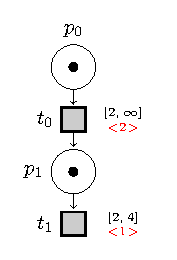
\includegraphics[keepaspectratio=true, width=0.2\textwidth]{time-pn.eps}
%   \caption[An example of time Petri net.]{An example of time Petri
%     net. The value of time counters appears between diamond brackets.}
%   \label{fig:tpn}
% \end{figure}
% For each sensitized transition associated with a time interval, time
% counters are incremented at a certain time step, previously defined by
% the designer. For instance, in the case of SITPNs, i.e. Petri nets
% used in the \hilecop{} methodology, the reference time step for the
% increment of time counters is the clock cycle.

% When a transition associated with a time interval is fired or
% disabled, a reset order is sent to the transition to set its time
% counter value to
% zero.
% In time Petri nets, a transition is firable if:
% \begin{itemize}[label=--]
% \item It is enabled.
% \item Its time counter value is within its time interval.
% \end{itemize}

% For instance, in Figure~\ref{fig:tpn}, only transition $t_0$ is
% firable.
% There are several possible firing policies for TPNs. Here, we will
% only consider the \textit{imperative} firing policy: as soon as a time
% counter reaches the lower bound of a time interval, the associated
% transition must be fired if all the other firability conditions are
% verified.

% Figure~\ref{fig:structural-conflict} illustrates the
% application of a priority relation to solve the effective conflict
% between two transitions.

% \begin{figure}[H]
%   \centering
%   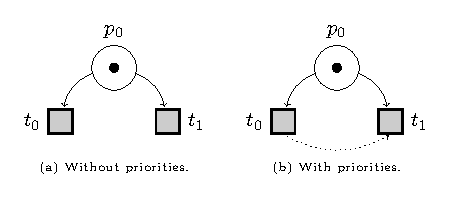
\includegraphics[keepaspectratio=true,width=.6\textwidth]{structural-conflict.eps}
%   \caption[An example of transitions in structural and effective
%   conflict.]{An example of transitions in structural and effective
%     conflict. In subfigure (b), the dotted arrow represents the
%     priority relation between $t_0$ and $t1$. The transition with the
%     highest firing priority is at the source of the arrow; here,
%     transition $t_0$.}
%   \label{fig:structural-conflict}
% \end{figure}

\subsection{Synchronous execution semantics}
\label{subsec:hpn-particularities}

% The aspect of SITPNs that constitutes the originality of the formalism
% compared to the standard PN semantics is its synchronous execution.
% The class of interpreted Petri nets increases the expressiveness of
% the \hilecop{} high-level models. However, to ensure the safe
% execution of functions after synthesis on a physical device, the whole
% system must be synchronized with a clock signal \cite{Leroux2014}. As
% a consequence, a clock signal regulates the evolution of SITPNS
% (i.e. it is a part of their semantics). 
 The SITPN semantics describes
the evolution of the state of an SITPN through a given number of clock
cycles; thus, we must first define the SITPN state structure. In what
follows, for a given $sitpn\in{}SITPN$, $T_i$ denotes the definition
domain of $I_s$, i.e. the set of transitions associated with a time
interval, referred to as \textit{time transitions}.

\begin{definition}[SITPN State]
  \label{def:sitpnstate}
  For a given $sitpn\in{}SITPN$, let $S(sitpn)$ be the set of possible
  states of $sitpn$. An SITPN state $s\in{}S(sitpn)$ is a tuple
  ${<}M,I,reset_t,ex,cond{>}$, where:
  \begin{enumerate}
  \item $M\in{}P\rightarrow\mathbb{N}$ is the current marking of sitpn.
  \item\label{item:sitpn-state-tc} $I\in{}T_i{}\rightarrow\mathbb{N}$
    is the function mapping time transitions to their current time
    counter value.
  \item\label{item:sitpn-state-rst}
    $reset_t\in{}T_i\rightarrow\mathbb{B}$ is the function mapping
    time transitions to time counter reset orders (defined as
    Booleans).
  \item $ex\in{}\mathcal{A}\sqcup\mathcal{F}\rightarrow\mathbb{B}$ is
    the function representing the current activation (resp. execution)
    state of actions (resp. functions).
  \item $cond\in\mathcal{C}\rightarrow\mathbb{B}$ is the function representing the
    current value of conditions (defined as Booleans).
  \end{enumerate}
\end{definition}

Considering the different classes of PNs that define SITPNs, the state
of a SITPN is characterized by its marking, the value of time
counters, the reset orders assigned to time counters, the
execution/activation status of actions/functions (Boolean values), and
the value of conditions (also Boolean). Regarding actions and
functions, note that we are only interested in the fact that a given
action/function is activated/executed but no more in actually
executing the associated operation. 

% Figure~\ref{fig:sync-exec} depicts the process of state evolution,
% following the clock signal.

% \begin{figure}[H]
%   \centering
%   
\includegraphics[keepaspectratio=true, width=.9\textwidth]{sync-exec.eps}
%   \caption{Evolution of an SITPN synchronized with a clock signal.}
%   \label{fig:sync-exec}
% \end{figure}

The evolution of the state of a SITPN is \textit{synchronized} with
two clock events: the rising edge and the falling edge of the clock
signal.
% As shown in Figure~\ref{fig:sync-exec}, the state evolution process
% of a SITPN is divided into two steps.
The rising edge of the clock signal triggers the marking update, which
is the consequence of transition firing; all time transitions that
have been fired or disabled by the firing process receive time counter
reset orders; all functions associated with fired transitions are
executed. Then, on the falling edge of the clock signal, the
environment provides a new value to each condition. The falling edge
triggers the evolution of the time counter values; values are
incremented, reset, or stalling in the case where a time counter has
reached the upper bound of its associated time interval (see the
following remark on locked time counters). Finally, all actions
associated with marked places are
activated. Figure~\ref{fig:sitpn-state-exec} gives an example of the
evolution of the state of a given SITPN through one clock cycle. % The
% aim of this figure and the explanation that follows is to give some
% hints to the reader about the semantics of SITPNs before giving its
% formal definition in Section~\ref{sec:sitpn-sem}.

\begin{figure}[H]
  \centering
  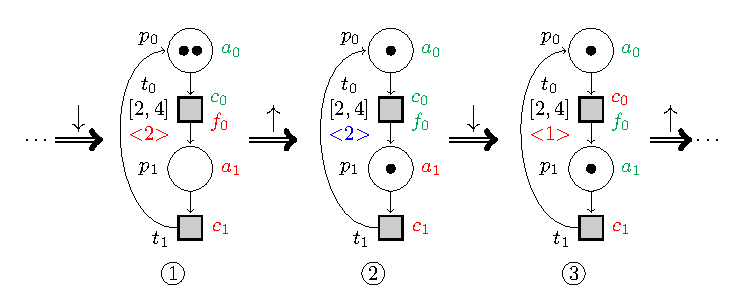
\includegraphics[keepaspectratio=true, width=.9\textwidth]{sitpn-state-evol.eps}
  \caption[Evolution of an SITPN over one clock cycle.]{Evolution of a
    SITPN over one clock cycle. Conditions appear in green when their
    value is \texttt{true} and in \textcolor{red}{red} otherwise;
    actions and functions appear in green  when they are
    activated/executed and in \textcolor{red}{red} otherwise; time
    counters appear in \textcolor{red}{red} and between diamond
    brackets; time counters appear in \textcolor{blue}{blue} when they
    receive reset orders.}
  \label{fig:sitpn-state-exec}
\end{figure}

From Step~1 to Step~2, the rising edge of the clock signal triggers
the SITPN state evolution. Here, transition $t_0$ is fired. At Step~1,
transition $t_0$ gathers all the necessary conditions to trigger the
firing process, namely:

\begin{itemize}[label=--]
\item $t_0$ is enabled by the current marking.
\item Condition $c_0$ is \texttt{true} (appears in green).
  
\item The value of $t_0$'s time counter is within the associated time
  interval ($2\in[2,4]$).
\end{itemize}

As a consequence, one token is consumed in place $p_0$ and one token
is produced in place $p_1$. Also, function $f_0$ is executed at the
occurrence of the rising edge of the clock signal, and thus, $f_0$
appears in green at Step~2. Due to the firing of $t_0$ at the rising
edge, a reset order is sent to the time counter of $t_0$, and it
appears in \textcolor{blue}{blue} at Step~2. From Step~2 to Step~3,
the falling edge updates the action activation status: $a_0$ stays
activated as place $p_0$ is still marked; $a_1$ becomes newly
activated as $p_1$ is marked. The value of time counters is updated:
$t_0$'s time counter is set to zero as the transition previously
received a reset order. However, as $t_0$ is still enabled by the new
marking, its time counter is incremented. Thus, the resulting time
counter value at Step~3 is of one (i.e. result of reset plus
increment). Also, the environment provides a new value to each
condition. As a consequence, condition $c_0$ takes the value
\texttt{false} and condition $c_1$ keeps the same value.

\paragraph{A remark on priorities}

The semantics of synchronous execution is that all transitions are
fired at the same time. In Figure~\ref{fig:double-consum}, transitions
$t_0$ and $t_1$ are both sensitized by place $p_0$, and consequently
are both fired at the same time. The system acts as if two tokens were
available in place $p_0$, one for the firing of $t_0$ and another for
the firing of $t_1$.

\begin{figure}[H]
  \centering
  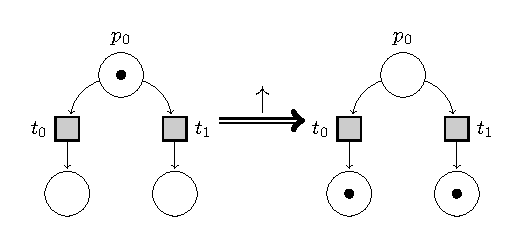
\includegraphics[keepaspectratio=true, width=.6\textwidth]{double-consum.eps}
  \caption[Double consumption of token in a SITPN.]{Double consumption
    of one token in a SITPN. On the left side, the current marking
    before the firing of $t_0$ and $t_1$; on the right side, the
    marking resulting of the firing of $t_0$ and $t_1$. The arrow
    indicates the occurrence of a rising edge that triggers the firing
    process.}
  \label{fig:double-consum}
\end{figure}

In the context of a SITPN, a branching like the one of
Figure~\ref{fig:sitpn-state-exec}, normally interpreted as a
disjunctive branching, takes the semantics of a conjunctive branching
when no priority are prescribed between the conflicting
transitions. To avoid the phenomenon of ``double consumption'' of
tokens, we enforce the resolution of any structural conflict by means
of mutual exclusion or through the application of priorities. This
policy about the resolution of structural conflicts is part of the
definition of a well-defined SITPN presented in
Section~\ref{sec:sitpn-wd}. The property of well-definition is
mandatory to produce safe models of digital systems.

When a structural conflict between transitions is solved with
priorities, the firing process follows a slightly different
mechanism. As illustrated in Figure~\ref{fig:resid-marking}, to
determine which transitions of $t_0$, $t_1$ and $t_2$ must be fired, a
\emph{residual marking} is computed by following the priority
order. For each transition of the group $t_0$, $t_1$ and $t_2$, the
residual marking represents the remaining tokens in $p_0$ after the
firing of transitions with a higher firing priority. Thus, in the
semantics of SITPNs, we add an extra condition to the firing of a
transition: to be fired, a transition must be:

\begin{itemize}[label=--]
\item enabled by the current marking
\item must have all its conditions valuated to \texttt{true}
\item must have its time counter within its time interval
\item \emph{and} must be enabled by the residual marking.
\end{itemize}

The computation of the residual marking only involves the consumption
phase of the firing process; tokens are withdrawn from places, but
none are generated.

\begin{figure}[H]
  \centering
  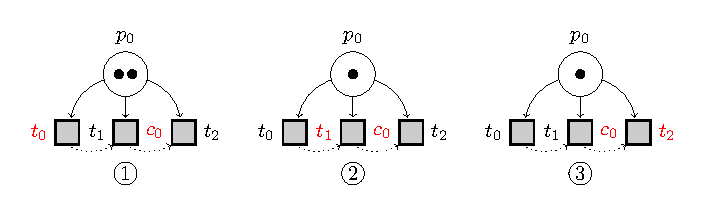
\includegraphics[keepaspectratio=true, width=.9\textwidth]{resid-marking.eps}
  \caption[Computation of the residual marking of a group of
  conflicting transitions.]{Computation of the residual marking for a
    group of conflicting transitions. At \circled{1}
    (resp. \circled{2} and \circled{3}), place $p_0$ holds the
    residual marking for transition $t_0$ (resp. $t_1$ and
    $t_2$). Condition $c_0$ is in \textcolor{red}{red} to indicate
    that its current value is \texttt{false}.}
  \label{fig:resid-marking}
\end{figure}

In Figure~\ref{fig:resid-marking}, the residual marking for $t_0$
corresponds to the marking obtained after the firing of all
transitions with a higher priority. As $t_0$ is the transition with
the highest firing priority, the residual marking for $t_0$ is equal
to the current marking. Transition $t_0$ gathers all the conditions to
be firable and is enabled by the residual marking; thus, $t_0$ will be
fired on the next rising edge. The residual marking for $t_1$ is the
marking obtained after the firing of $t_0$, i.e. the only transition
with a higher priority. As illustrated at \circled{2}, $t_1$ is
enabled by the residual marking. However, $t_1$ does not gather all
the conditions to be firable as the value of condition $c_0$ is
\texttt{false}. Thus, $t_1$ will not be fired on the new rising
edge. The residual marking for $t_2$ is obtained after the firing of
$t_0$ only. Even though transition $t_1$ has a higher firing priority
than $t_2$, $t_1$ is not a member of the set of fired transitions.
Thus, $t_1$ is not taken into account in the computation of the
residual marking for $t_2$. The residual marking at \circled{3}
enables transition $t_2$, and as $t_2$ gathers all the conditions to
be firable, then $t_2$ will be fired on the next rising edge.

% \paragraph{Locked time counters}

% SITPNs inherit the properties of time PNs and interpreted PNs. The
% phenomenon of \emph{locked} time counters is a consequence of this
% inheritance. As illustrated in Figure~\ref{fig:locked-tc}, the value
% of a time counter can overreach the upper bound of its associated time
% interval. This situation can only arise if a condition hinders the
% firing of a given transition while the considered transition is still
% enabled by the marking. As a consequence, the time counter will be
% incremented at every clock cycle until the upper bound of the time
% interval is overreached. Then, at this point, the time counter is said
% to be \emph{locked} and its value will no more evolve.

% \begin{figure}[H]
%   \centering
%   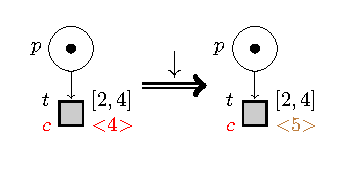
\includegraphics[keepaspectratio=true, width=.45\textwidth]{locked-tc.eps}
%   \caption[An example of locked time counter.]{An example of locked
%     time counter. Condition $c$ is equal to \texttt{false} and thus
%     appears in \textcolor{red}{red}.}
%   \label{fig:locked-tc}
% \end{figure}

% In Figure~\ref{fig:locked-tc}, condition $c$ is valuated to
% \texttt{false} before the falling edge of the clock signal. Thus,
% transition $t$ can not be fired but is still enabled by the
% marking. On the next falling edge, the time counter of transition $t$
% is incremented and overreaches the upper bound of interval $[2,4]$ and
% thus becomes locked. If the designer of the model has not anticipated
% the case of a locked time counter, and has not provided an alternative
% to disable place $p$ in that case, then the transition $t$ will never
% be firable again.

Regarding conditions, we consider that they directly receive their
value from an environment that would have computed in our stead the
values of the Boolean expressions. Thus, we no more have to consider
the Boolean expressions associated with conditions, and only have to
rely on the values given by the environment. Regarding actions and
functions, we are only interested in the fact that a given
action/function is activated/executed but no more in actually
executing the associated operation.

\section{A target language: \hvhdl{}}
\label{sec:hvhdl}

\section{Model-to-text transformation}
\label{sec:m2t}

\section{Proof of semantic preservation}
\label{sec:proof}

\section{Conclusion}
\label{sec:concl}


\bibliography{references}

\end{document}
